 \documentclass[12pt,a4paper]{article}
%\usepackage{hyperref} % Use the Charter font for the document text
%\usepackage[UTF8]{ctex}
\usepackage{jheppub}

\usepackage{amsfonts,amssymb,amsmath}
\usepackage{mathtools}
\usepackage{tikz-cd}
\usepackage{tikz}
\usepackage{alltt}
\usepackage{amsfonts}
\usepackage{amsmath}
\usepackage{amssymb}
\usepackage{amsthm}
\usepackage{booktabs}
\usepackage{caption}
\usepackage{enumitem}
\usepackage{fancyhdr}
\usepackage{graphicx}
\usepackage{mathdots}
\usepackage{mathtools}
\usepackage{microtype}
\usepackage{multirow}
\usepackage{pdflscape}
\usepackage{pgfplots}
\usepackage{siunitx}
\usepackage{slashed}
\usepackage{tabularx}
\usepackage{tikz}
\usepackage{tkz-euclide}
\usepackage[normalem]{ulem}
\usepackage[all]{xy}
\usepackage{imakeidx}

\usepackage{wrapfig}

%%\input{dummy.tex}
%
%%%% tikzセッティング %%%%%%%%%%%%%%%%%%%%%%%%%%%%%%%
%\usepackage[dvipdfmx]{graphicx}
%\usepackage{tikz}
%\usetikzlibrary{arrows,shapes,patterns,snakes,calc}
%%\input{arrowsnew}
%\usetikzlibrary{decorations.markings}
%\usetikzlibrary{positioning}
%%%% end of tikz %%%%%%%%%%%%%%%%%%%%%%%%%%%%%%%%%%%%
%
%\usepackage[hang,bf,figurename=Fig.\ , tablename=Table\ ,margin=1cm]{caption}
%\renewcommand{\captionfont}{\footnotesize}

%%% listingsセッティング %%%%%%%%%%%%%%%%%%%%%%%%%%%
%\usepackage{listings, jlisting}
%\renewcommand{\lstlistingname}{Code}
%\definecolor{mygreen}{rgb}{0,0.6,0}
%\definecolor{mygray}{rgb}{0.5,0.5,0.5}
%\definecolor{mymauve}{rgb}{0.58,0,0.82}
%
%\lstset{ %
%  % language=Octave,                 % the language of the code
%  backgroundcolor=\color{white},   % choose the background color; you must add \usepackage{color} or \usepackage{xcolor}
%  basicstyle=\footnotesize,        % the size of the fonts that are used for the code
%  breakatwhitespace=false,         % sets if automatic breaks should only happen at whitespace
%  breaklines=true,                 % sets automatic line breaking
%  captionpos=t,                    % sets the caption-position to bottom
%  commentstyle=\color{mygreen},    % comment style
%  deletekeywords={...},            % if you want to delete keywords from the given language
%  escapeinside={\%*}{*)},          % if you want to add LaTeX within your code
%  extendedchars=true,              % lets you use non-ASCII characters; for 8-bits encodings only, does not work with UTF-8
%  frame=single,                    % adds a frame around the code
%  keepspaces=true,                 % keeps spaces in text, useful for keeping indentation of code (possibly needs columns=flexible)
%  keywordstyle=\color{blue},       % keyword style
%  morekeywords={*,...},            % if you want to add more keywords to the set
%  numbers=left,                    % where to put the line-numbers; possible values are (none, left, right)
%  numbersep=5pt,                   % how far the line-numbers are from the code
%  numberstyle=\tiny\color{mygray}, % the style that is used for the line-numbers
%  rulecolor=\color{black},         % if not set, the frame-color may be changed on line-breaks within not-black text (e.g. comments (green here))
%  showspaces=false,                % show spaces everywhere adding particular underscores; it overrides 'showstringspaces'
%  showstringspaces=false,          % underline spaces within strings only
%  showtabs=false,                  % show tabs within strings adding particular underscores
%  stepnumber=1,                    % the step between two line-numbers. If it's 1, each line will be numbered
%  stringstyle=\color{mymauve},     % string literal style
%  tabsize=2,                       % sets default tabsize to 2 spaces
%  title=\lstname                   % show the filename of files included with \lstinputlisting; also try caption instead of title
%}
%%% ned of listings セッティング %%%%%%%%%%%%%%%%%%%%%%%%%%%

%
%\pdfstringdefDisableCommands{%
%    \renewcommand*{\bm}[1]{#1}%
%    % any other necessary redefinitions 
%}

%%%今村セッテッティング%%%%%%%%%%%%%%%%%%%%%%%%%%%%%
\newcommand{\CC}{\mathbb{C}}
\newcommand{\ZZ}{\mathbb{Z}}
\newcommand{\RR}{\mathbb{R}}
\newcommand{\HH}{\mathbb{H}}

\newcommand{\hf}{\frac{1}{2}}
\newcommand{\tr}{{\rm tr}}
\newcommand{\ind}{{\rm ind}}
\newcommand{\ol}{\overline}
\newcommand{\ul}{\underline}
\newcommand{\up}{\uparrow}
\newcommand{\dn}{\downarrow}
\newcommand{\wt}{\widetilde}
\newcommand{\ra}{\rightarrow}
\newcommand{\wh}{\widehat}


%%%横山セッティング%%%%%%%%%%%%%%%%%%%%%%%%%%%%%%%%%
\newcommand{\NN}{\mathcal{N}\!}
\newcommand{\DD}{\mathcal{D}}
\newcommand{\UU}{U(1)}
\newcommand{\dd}{\mathrm{d}}
\renewcommand{\SS}{\mathbf{S}}
\renewcommand{\Im}{\mathrm{Im}}
\renewcommand{\Re}{\mathrm{Re}}
%\renewcommand{\<}{\langle}
%\renewcommand{\>}{\rangle}
\newcommand{\Tr}{{\rm Tr}}

\renewcommand{\r}{\mathrm}

\newcommand{\sign}{\mathrm{sign}}

\newcommand{\lra}{\leftrightarrow}
\newcommand{\LL}{\mathcal{L}}
\newcommand{\la}{\leftarrow}
\newcommand{\ro}{\sqrt}
\newcommand{\Ra}{\Rightarrow}
\newcommand{\Pexp}{\mathrm{Pexp}}

\newcommand{\nn}{\nonumber \cr}
%\newcommand{\1}{\mbox{1}\hspace{-0.25em}\mbox{l}}

%数字のみ対応
\newcommand{\Maru}[1]{\ooalign{
\ifnum#1<10 \hfil\resizebox{.9\width}{.85\height}{#1}\hfil
\else
\hfil\resizebox{.6\width}{.8\height}{#1}\hfil
\fi
\crcr
\raise.1ex\hbox{$\bigcirc$}}}

%全文字対応
\newcommand{\maru}[1]{\ooalign{
\hfil\resizebox{.8\width}{\height}{#1}\hfil
\crcr
\raise.1ex\hbox{\large$\bigcirc$}}}


\newcommand{\nord}[1]{\vcentcolon\mathrel{#1}\vcentcolon}
\providecommand{\vcentcolon}{\mathrel{\mathop{:}}}


\def\P{\mathop{\cal P}}
\def\diag{\mathop{\rm diag}}


\def\Re{\mathop{\rm Re}\nolimits}
\def\Im{\mathop{\rm Im}\nolimits}
\def\Det{\mathop{\rm Det}\nolimits}
\def\sign{\mathop{\rm sign}\nolimits}
%
%
%%%% rap %%% - make two letters overlap
%\newcommand{\rap}[2]
%{\setbox1=\hbox{#1}%
%\setbox2=\hbox to\wd1{\hss #2\hss}%
%\mbox{\rlap{\box1}\box2}}
%
%%\newcommand{\sla}[1]{\rap{$#1$}{/}}
%\newcommand{\sla}[1]{\rap{$#1$}{$\backslash$}}
%
%
%\def\DY#1{{\MyGreen [DY: #1]}}
%\newcommand{\MyGreen}{\color [rgb]{0,0.7,0}}
%
%\usepackage[vcentermath]{youngtab}
% \Yboxdim4pt
\newcommand{\Y}{\yng}
\newcommand{\Young}{}


%%%%title def%%%%%%%%%%%%%%%%%%%%%%%%%%%%%%%%%%%%%%%%%%%%%%%
%
%\makeatletter
%\def\maketitle{
%\noindent
%{\Large \@title \par\vskip 2pt}
%\noindent
%{\large \@date \hspace{4pt} \@author}
%%\cr[-2pt]
%%\noindent------------------------------------------------------------------------------------------
%\par\vskip 1.5em
%}
%
%\author{横山 大輔}
%\date{\today}
%%%%本文%%%%%%%%%%%%%%%%%%%%%%%%%%%%%%%%%%%%%%%%%%%%%%%%%%%%%%%%

% \title{\centerline{Lecture 2}}
\begin{document}
% \maketitle
% \begin{abstract}

% \end{abstract}
% \tableofcontents
%
  \pagestyle{fancy}
  \renewcommand{\headrulewidth}{0.0pt}
  \rhead{}
  \lhead{}
  \cfoot{[\ \scshape\oldstylenums{\thepage}\ / %
    \scshape\oldstylenums{\pageref{lastpage}} ]}
%  \rfoot{\@author}

% \setcounter{section}{}
% \setcounter{subsection}{}
% \setcounter{subsubsection}{}

\centerline{\Large \bf  Lecture 2}

\vspace{12pt}
Note that in this lecture we use $\alpha'$ rather than string tension $T = \frac{1}{2\pi\alpha'}$.
World-sheet(WS) index here is denoted by $a, b$ rather than $\alpha, \beta$.
$h_{ab}$ is WS metric; do not confuse with the induced metric $h_{\alpha\beta} = \eta_{\mu\nu} \partial_\alpha X^\mu \partial_\beta X^\nu$
used in the last lecture.
Convention in this note basically follows Polchinski's one, though
we adopt slightly different normalization for Noether current in Sec.~2.4.
\vspace{-12pt}

\section{Towards string interaction}

What we have learnt is
\begin{itemize}
% \item Nambu-Goto action $\sim$ String sigma model (by introducing),
% \item Weyl invariance (inv) $\times$ world-sheet (WS) diffeomorphism (diff) is important,
 \item Mass spectrum of a string by light-cone quantization in flat space-time (ST).
\end{itemize}
What we have NOT learnt is
\begin{itemize}
 \item string interactions,
 \item extension to curved background (curved ST).
\end{itemize}
Especially because of the first reason(string interaction)
we want to express our analysis in terms of \textit{path integral},
which is more natural to illustrate string interaction.
(If you are not familiar with path integral, consult the appendix of Polchinski Vol.1. for derivation.)
See Fig.~\ref{fig1}, which is a naive but appropriate extension from quantum field theory (QFT) interaction to string interaction.
\begin{figure}[htb]
 \centerline{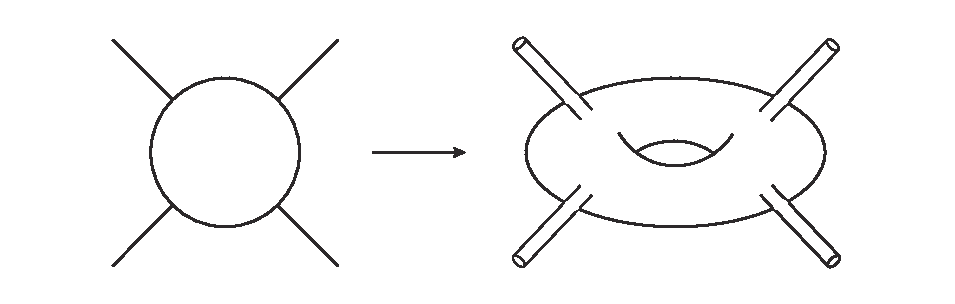
\includegraphics[width=250pt]{fig1}}
 \caption{A Feynman diagram of QFT (left) and a string interaction diagram (right). Each end of the cylinders connecting to the torus(Riemann surface) in the string interaction diagram corresponds to an initial/final state.}
 \label{fig1}
\end{figure}
Each end of the cylinders in the Figure corresponds to an initial/final state of string.
It is quite cumbersome to use \textit{state} expression.
Instead, we will use vertex operator $\wh V$ to express those states, which is explained in the following subsection.
Given that we adopt the operator expression the string interaction is written as in Fig.~\ref{fig2} as well as
\begin{align}\nonumber
 A_n = \sum_g \int \left(\DD h_{ab}\right)_{g,n} \int \DD X^\mu e^{-S_\sigma [X^\mu,h_{ab}]} \wh V_1 \cdots \wh V_n \ ,
\end{align}
where $n$ is the number of in-coming/out-going strings, and $g$ is the number of holes(genus) of the Riemann surface (genus is $1$ in the figures).
\begin{figure}[htb]
 \centerline{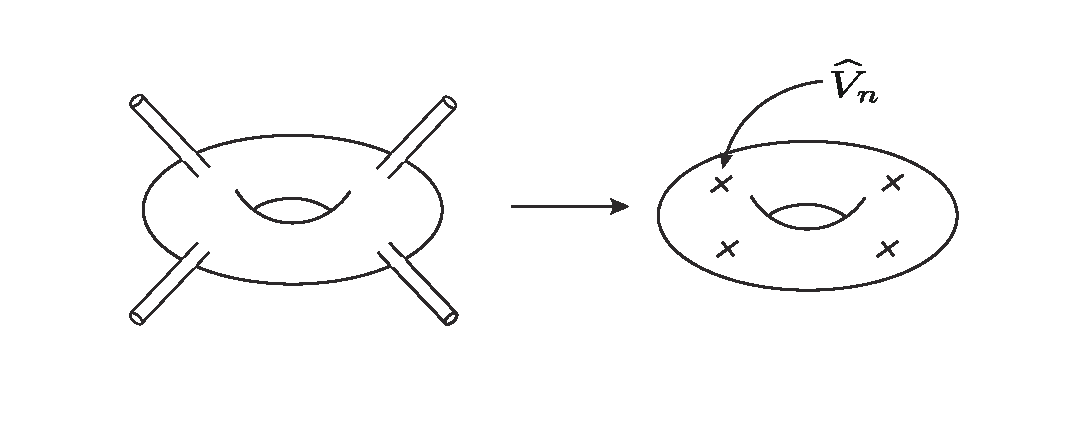
\includegraphics[width=250pt]{fig2}}
 \caption{String interaction in state expression (left) and operator expression (right).}
 \label{fig2}
\end{figure}

\subsection{Path integral method}

% As a short goal of studying string theory, we want to know the spectra of a closed/open string,
% and how to describe string interactions.

% The operator analysis is a tool to achieve these purposes.
% This is because the string world sheet theory is a conformal field theory


In path integral method expectation values(partition function, 2pt func etc.) are given in the following form
\begin{align}\nonumber
 \langle \mathcal O[X] \rangle = \int \DD X e^{iS[X]} \mathcal O [X] \ ,  \qquad
 S = \frac{1}{4\pi \alpha'} \int d\sigma d\tau \left\{ \left(\partial_\tau X\right)^2 -\left(\partial_\sigma X\right)^2\right\} \ ,
\end{align}
where $\mathcal O$ is an arbitrary operator (eg. for partition function $\mathcal O = 1$, for 2pt func $\mathcal O = X^\mu X^\nu$).
Note that we often omit the (super-)sub-script $\mu$ if it is not crucial.
% $S[X]$ etc. are called functional.
We usually \textbf{Wick rotate} ($\tau \ra -it$) the theory so that it converges.
\begin{align}\nonumber
 \langle \mathcal O[X] \rangle = \int \DD X e^{-S_E[X]} \mathcal O [X] \ ,  \qquad
 S_E = \frac{1}{4\pi \alpha'} \int d\sigma dt \left\{ \left(\partial_t X\right)^2 +\left(\partial_\sigma X\right)^2\right\} \ .
\end{align}
The subscript $E$ will be omitted hereafter, and we will always work in the WS Euclidean signature.


(Even if you do not know path integral well) What we need to understand (at least for today) is that we can manipulate it as like normal integral:
\begin{itemize}
 \item total derivative vanishes (assumption)
  \begin{align}\nonumber
   0 = \int \DD X \frac{\delta}{\delta X} \left( e^{-S_E[X]} \mathcal O [X] \right) \ .
  \end{align}
% \item it commutes with derivatives
\end{itemize}
Note that with subscripts the functional derivative gives
\begin{align}\nonumber
 \frac{\delta X^\mu (w)}{\delta X^\nu (z)} = \delta^\mu_\nu \delta^2(z-w) \ .
\end{align}

\subsection{State-operator correspondence}


As we have seen the string sigma model is Weyl invariant:
\begin{align}\nonumber
 S_\sigma \left[ X^\mu, h_{ab} \right] = S_\sigma \left[ X^\mu, e^{\phi(\sigma)} h_{ab} \right] \ .
\end{align}
This (and together with WS diff) can be regarded as a property of the matter theory as we saw in the previous lecture,
and we say that matter theory of $X$ is conformally invariant or the matter theory is a conformal field theory (CFT).
We can use this freedom to set WS to be $\RR^2$ (recall that the topology of (closed) string is cylinder).
\begin{align}\nonumber
 \RR^2:  \quad ds^2 &= dx^2 +dy^2 = dr^2 +r^2 d\theta^2 \nn
 &= r^2 \left[ d\left(\log r\right)^2 +d\theta^2 \right] \ , \nn
 \textrm{Cylinder} : \quad ds^2 &= dt^2 +d\sigma^2 \ ,
\end{align}
where the overall factor $r^2$ in $\RR^2$ is identified with the Weyl factor $e^{\phi(\sigma)}$, and can be removed.
So we can identify:
\begin{align}\nonumber
 t = \log r \ ,  \qquad  \sigma = -\theta \ .
\end{align}
The reason for the minus sign will be clear later.
This identification tells us that there is a correspondence between
\begin{itemize}
 \item CFT on a semi-infinite cylinder $(\sigma, t;\ t \le 0)$ , and
 \item CFT on a disk $(x^2+y^2 \le 1)$ with the origin removed  ,
\end{itemize}
provided that we choose the boundary conditions to be the same.
Especially, the initial \textit{state} of the string ($t = -\infty$) corresponds to a \textit{local operator}
inserted at the origin, which is called vertex operator (see Fig.~\ref{fig3}).
\begin{figure}[htb]
 \centerline{\includegraphics[width=250pt]{fig3}}
 \caption{State-operator correspondence. Initial state(red circle) is mapped to a local operator(red dot) at the origin.}
 \label{fig3}
\end{figure}
This is the state-operator correspondence and we will express string states by the vertex operators
(see again Fig.~\ref{fig2}).


Now you may wonder if there is any way to express commutation relations in terms of operators
so that we can do parallel procedures of the canonical quantization in terms of operators.
This is what we do in the next section.




\section{Conformal field theory in 2d}


We will learn operator analysis of 2d conformal field theory (CFT), including OPE, Ward-Takahashi identity etc.,
and we will see Virasoro algebra, which is associated to the conformal symmetry.


% As we have learnt in the last lecture the conformal transformations are arbitrary holomorphic/anti-holomorphic local translation.
% The action is invariant under the transformation






\subsection{Massless scalar theory in 2d}


We study massless scalar fields as the easiest example.
We adopt Euclidean metric $\eta_{ab} = \diag(+,+)$, though the procedure is parallel for Lorentz metric.
The action of massless scalar fields $X^\mu$ ($\mu = 1, 2,\cdots,D$) is given by
\begin{align}\nonumber
 S_\mathrm{} = \frac{1}{4\pi\alpha'} \int d^2x \ \left( \partial_1 X \cdot \partial_1 X +\partial_2 X \cdot \partial_2 X \right) \ ,
\end{align}
where $d^2x = dx_1dx_2$, $x_1 = x$, $x_2 =y$, and $\partial_i = \frac{\partial}{\partial x_i}$.
(The subscript E will be omitted hereafter.)


It is convenient to introduce complex coordinates and
accordingly vectors, metric etc.
\begin{itemize}

 \item Coordinates
  \begin{align}\nonumber
   z = x +iy \ , \qquad  \ol z = x -iy \ .
  \end{align}

 \item Derivatives
  \begin{align}\nonumber
   \partial \equiv \partial_z = \frac{\partial}{\partial z} = \frac{1}{2} \left( \partial_1 -i\partial_2 \right) \ ,  \quad
   \ol\partial \equiv \partial_{\ol z} = \frac{\partial}{\partial \ol z} = \frac{1}{2} \left( \partial_1 +i\partial_2 \right) \ ,
  \end{align}
       so that $\partial z = 1$, $\partial \ol z = 0$, $\ol\partial z = 0$, $\ol\partial \ol z = 1$.

 \item Vectors
  \begin{align}\nonumber
   v^z = v^1 +iv^2 \ , \qquad  v^{\ol z} = v^1 -iv^2 \ .
  \end{align}

 \item Metric
  \begin{align}\nonumber
   h_{z\ol z} = h_{\ol z z} = \frac{1}{2} \ , \quad h_{z z} = h_{\ol z\ol z} = 0 \ , \quad
   h^{z\ol z} = h^{\ol z z} = 2 \ , \quad h^{z z} = h^{\ol z\ol z} = 0 \ .
  \end{align}
  So lower-index vectors are $v_z = h_{z\ol z} v^{\ol z} = \frac{1}{2} (v^1-iv^2) $ etc.
 \item Integration measure
  \begin{align}\nonumber
   d^2z = dzd\ol z = 2 dx dy = 2 d^2 x \ ,
  \end{align}
       where the factor $2$ comes from the Jacobian.
       One can also write
  \begin{align}\nonumber
   \sqrt{h} d^2 z = \sqrt{|\det h_{ab}|} d^2 z = d^2x \ .
  \end{align}

 \item Delta function
  \begin{align}\nonumber
   \delta^2(z) = \delta(z)\delta(\ol z) = \frac{1}{2} \delta(x)\delta(y) = \frac{1}{2} \delta^2(x) \ ,
  \end{align}
       so that
  \begin{align}\nonumber
   1= \int d^2z\ \delta^2(z) = \int d^2 x\ \delta^2 (x) \ .
  \end{align}
\end{itemize}
Note that although $z$ and $\ol z$ are complex conjugate of each other,
we will treat them as independent complex numbers.
% Note that we are following Polchinski's notations rather than Hosomichi's.

\textbf{Stokes' theorem} (it is called Green's theorem in 2d) will be used frequently.
\begin{align}\nonumber
 \int_D d^2z \left( \partial \ol V + \ol\partial V\right)
 = \frac{1}{i} \oint_{\partial D} \left( V dz - \ol V d\ol z \right) \ ,
\end{align}
where $D$ is an arbitrary region (typically small disk) and $\partial D$ is its boundary.
$V$ and $\ol V$ are independent factor.
% \DY{Derivation of this form from normal Green's theorem could be exercise.}
Using the Stokes' theorem one can prove following equation.
\begin{align}
 \partial\ol\partial \log |z|^2 =2\pi \delta^2(z) \ .
 \label{eq:deltaFunc}
\end{align}
(Keep this in mind. We will use this later.)



With the complex coordinate convention, the action becomes
\begin{align}\nonumber
 S = \frac{1}{2\pi\alpha'} \int d^2 z\ \partial X \cdot \ol\partial X
 \quad
 \left( = \frac{1}{4\pi \alpha'}\int \sqrt h d^2z\ h^{ab} \partial_a X \cdot \partial_b X \right) \ .
\end{align}
The equation of motion (E.O.M) is given by
\begin{align}\nonumber
 \delta S &= \frac{1}{2\pi \alpha'} \int d^2z \left( \partial X \cdot \ol\partial (\delta X) +\partial (\delta X) \cdot \ol\partial X \right)  \nn
 &= -\frac{1}{\pi \alpha'} \int d^2z\ \delta X \cdot \partial\ol\partial X  =0 \ ,  \nn
 \therefore & \quad \partial\ol\partial X^\mu = 0 \ .
\end{align}
General solution to the E.O.M is
\begin{align}\nonumber
 X^\mu(z,\ol z) &= X_R^\mu (z) +X_L^\mu (\ol z)   ,   \cr
 X_R^\mu (z) &= \frac{1}{2}x^\mu -i \frac{\alpha'}{2} p^\mu \log z +i \sqrt{ \frac{\alpha'}{2} } \sum_{n \neq 0} \frac{1}{n} \frac{\alpha_n^\mu}{z^n} \ , \cr
 X_L^\mu (\ol z) &= \left. X_R^\mu (\ol z) \right|_{\alpha_n \ra \wt \alpha_n} \ .
\end{align}
Notice that
\begin{align}\nonumber
 z &= r e^{i\theta} = e^{\log r +i\theta} = e^{i\tau -i\theta}  \nn
   &= e^{i\sigma^-} \ ,  \cr
 \ol z &= e^{i\sigma^+} \ ,
\end{align}
and compare to
\begin{align}\nonumber
 X^\mu_R(\sigma^-) &= \frac{1}{2} x^\mu + \frac{1}{2} \alpha' p^\mu \,\sigma^- + i\sqrt{\frac{\alpha'}{2}}\sum_{n\neq 0}
\frac{1}{n}\,{\alpha}_n^\mu\, e^{-in\sigma^-} \ .
\end{align}




\subsection{Operator analysis (Path integral quantization)}



Let us consider quantum version of the E.O.M by using a path integral formulation.
% Correlation function of an operator $\mathcal O$ is given by a path integral
% \begin{align}\nonumber
%  \langle \mathcal O \rangle = \int \mathcal D \Phi e^{-S[\Phi]} \mathcal O[\Phi]  .
% \end{align}
As like a normal integral we assume that ``total derivative'' vanishes in path integral.
For example, in the massless free scalar case we have
\begin{align}\nonumber
 0 = \int \mathcal D X \ \frac{\delta}{\delta X} e^{-S[X]} = \int \mathcal D X \ e^{-S[X]} \frac{1}{\pi\alpha'}\partial\ol\partial X
 = \frac{1}{\pi\alpha'} \langle \partial\ol\partial X \rangle \ ,
\end{align}
which is nothing but Ehrenfest's theorem.
The E.O.M is satisfied as an operator equation if there is no other operator nearby.


Furthermore, the same procedure can be done with operator insertions.
The easiest example is
\begin{align}\nonumber
 0 = \int \mathcal D X \ \frac{\delta}{\delta X_\mu (z,\ol z)} \left(e^{-S[X]} X^\nu (w,\ol w) \right)
 = \langle \frac{1}{\pi\alpha'}\partial_z\partial_{\ol z} X^\mu (z,\bar z) X^\nu(w,\bar w) + \eta^{\mu\nu}\delta^2(z-w) \rangle \ .
\end{align}
Therefore,
\begin{align}\nonumber
 \partial\ol\partial X^\mu (z,\bar z) X^\nu(w,\bar w) = -\pi\alpha' \eta^{\mu\nu}\delta^2(z-w) \ ,
\end{align}
where note that this is operator equation (not classical equation) and we simply omitted $\langle \rangle$ symbols.
The right hand side is understood due to a quantum effect.

Recalling Eq.~(\ref{eq:deltaFunc}) we have
\begin{align}\nonumber
 X(z,\bar z)^\mu X^\nu(w,\bar w) = -\frac{\alpha'}{2} \eta^{\mu\nu} \log |z-w|^2 + \nord{X(z,\bar z)X(w,\bar w)} \ ,
\end{align}
where we introduced normal ordering $\nord{\mathcal O}$, meaning that the divergence at $z \ra w$ has been subtracted.
We also write it as follows.
\begin{align}\nonumber
 \nord{X^\mu(z,\bar z)X^\nu(w,\bar w)} = X^\mu(z,\bar z)X^\nu(w,\bar w) -\eta^{\mu\nu}G(z,w) \ ,
\end{align}
where $G(z,w) = -\frac{\alpha'}{2} \log|z-w|^2$.
Notice that
\begin{align}
 \partial_z \partial_{\ol z} \nord{X(z,\bar z)X(w,\bar w)} = 0 \ .
 \label{eq:normalEOM}
\end{align}
As we will see later the divergent term is important and meaningful.
This is why it is convenient to introduce the normal ordering so that we can separate the divergent terms from the other.



For an arbitrary functional of fields the OPE is expressed as follows.
% \begin{align}\nonumber
%  \nord{X_1 X_2 \cdots X_n} = X_1 X_2 \cdots X_n -\sum_\textrm{1 pair} G_{i_1 i_2} X_{i_3} \cdots X_{i_n}
%  +\sum_\textrm{2 pairs} G_{i_1 i_2} G_{i_3 i_4} X_{i_5} \cdots X_{i_n} -+ \cdots  .
% \end{align}
\begin{align}\nonumber
 \nord{f[X]} = \exp \left[ -\frac{1}{2} \int d^2z d^2w\ G(z,w) \frac{\delta}{\delta X^\mu(z,\bar z)} \frac{\delta}{\delta X_\mu(w,\bar w)} \right]
 f[X] \ .
\end{align}
For example,
\begin{align}\nonumber
 \nord{X_1X_2X_3X_4X_5} =& X_1X_2X_3X_4X_5 -\left( G_{12}X_3X_4X_5 +\cdots \right)_\textrm{10 terms}  \nn
 &+\left( G_{12}G_{34}X_5 +\cdots \right)_\textrm{15 terms} \ ,
\end{align}
where $X_i=X(z_i)$ and $G_{ij} = G(z_i,z_j)$.


Multiplication of normal ordered product is given as follows.
\begin{align}\nonumber
 \nord{f[X]} \nord{g[X]} = \exp \left[ \int d^2z d^2w\ G(z,w) \left. \frac{\delta}{\delta X^\mu(z,\bar z)} \right|_{f} \left. \frac{\delta}{\delta X_\mu(w,\bar w)} \right|_{g} \right] \nord{fg[X]} \ .
\end{align}
Example 1:
\begin{align}\nonumber
 \nord{ \partial X(z,\bar z)} \nord{ X(w,\bar w)} = \nord{\partial X(z,\bar z) X (w,\bar w)} +\partial_z G(z,w)  
 = \nord{\partial X (z,\bar z) X (w,\bar w)} -\frac{\alpha'}{2} \frac{1}{z-w} \ .
\end{align}
Example 2:
\begin{align}\nonumber
 \nord{e^{ik\cdot X(z,\bar z)}} \nord{e^{ik'\cdot X(w,\bar w)}} &= \exp\left[ (ik) \cdot (ik') \left( -\frac{\alpha'}{2} \log|z-w|^2 \right)\right]
 \nord{e^{ik\cdot X(z,\bar z) +ik'\cdot X(w,\bar w)}} \nn &= |z-w|^{\alpha'k\cdot k'} \nord{e^{ik\cdot X(z,\bar z) +ik'\cdot X(w,\bar w)}} \ .
\end{align}






\subsection{Operator product expansion (OPE)}


% \DY{これを言うためには operator であること、つまり quantum field theory であることを言わなければならない。}
In general field theory, product of a pair of fields can be expanded by a single operator
\begin{align}\nonumber
 \Phi^i (z) \Phi^j (w) = \sum_{k} C^{ij}_k(z-w) \Phi^k (w) \ .
\end{align}
% We omit the second variable $\ol z$ hereafter (namely, $\Phi(z)=\Phi(z,\ol z)$).
Note that in 2d CFT language any local operator is regarded as an independent field (e.g. $\Phi = X, \partial X, \nord{XX}$ etc.).


Typically, for a massless free scalar field theory we have
\begin{align}\nonumber
 &X^\mu (z,\ol z) X^\nu (w,\ol w) =  -\frac{\alpha'}{2} \eta^{\mu\nu} \log |z-w|^2 +\nord{X^\mu X^\nu (w,\ol w)}  \nn
 &\qquad +\sum_{k=1}^\infty \frac{1}{k!} \left\{ (z-w)^k  \nord{\partial^k X^\mu X^\nu (w, \ol w)}
 +(\ol z-\ol w)^k  \nord{\ol\partial^k X^\mu X^\nu (w, \ol w)}\right\} \ .
\end{align}
The second and the third terms of RHS can be understood as Taylor expansion of $\nord{X(z)X(w)}$ in terms of $z$. Mixing terms ($\nord{\partial^m\ol\partial^n X X}$) vanish due to ``E.O.M'', Eq.~(\ref{eq:normalEOM}).


As we will see, only the divergent term is important.
We will introduce $\sim$ that is define as ``equal up to non-divergent term''
so that we can forget about non-divergent terms.
For example
\begin{align}\nonumber
 X^\mu (z,\ol z) X^\nu (w,\ol w) \sim  -\frac{\alpha'}{2} \eta^{\mu\nu} \log |z-w|^2 \ .
\end{align}



\subsection{Noether's theorem and Ward-Takahashi identities}

When an action is invariant under a certain transformation $\delta$ (namely, $\delta S = 0$)
we say the theory has a (classical) symmetry.
Furthermore, the measure of the path integral is also invariant under the
transformation we say the theory has a symmetry at quantum level.
On the other hand, if the measure is not invariant, then, we say the theory has anomaly and/or the symmetry is anomalous.
It is non-trivial to see if the theory has anomaly or not.

If the theory has a symmetry there is a corresponding conserved current $j^a$
and the space integral of its time component is the conserved charge $Q=\int_\textrm{space} j^0$, which generate the symmetry $\delta X = [Q, X]$.
The current can be derived by Noether's procedure.
Even if you are not familiar with the Noether's theorem
we will see alternative method.


Let $\delta$ be a symmetry $\delta S = 0$ and assume it acts on a field as follows: $\delta X (z) = \epsilon (\cdots) $, where $\epsilon$ is a small parameter.
If we promote the parameter to be WS coordinate dependent (i.e. $\wh \delta X = \epsilon(z,\ol z) (\cdots)$), then $\wh \delta S$ is no longer zero but has to take the following form.
\begin{align}\nonumber
 \wh\delta S = \int \frac{d^2 x}{2\pi} \epsilon(x,y) \partial_a j^a
 = \int \frac{d^2z}{2\pi} \epsilon(z, \ol z)
 \left( \partial \ol j +\ol\partial j \right) \ ,
\end{align}
where we introduced $j = j_{z}$ and $\ol j = j_{\ol z}$.
If the parameter is constant $\delta S = (\textrm{total derivative}) = 0$.
\textbf{ $j^a$ is Noether current}.
Noether current is conserved, which means that $\partial_a j^a = 0$ under assumption of E.O.M.
This implies that $j$($\ol j$) is a holomorphic(anti-holomorphic) function of $z$.
Indeed, this is true for all the example we will see.


\subsubsection*{Ward-Takahashi identity}

Now let us study the transformation of  a point operator $\mathcal{O}[X](w,\ol w)$ under the symmetry $\delta$. For this purpose, 
we set
\begin{align}\nonumber
 \epsilon(z,\ol z) =
 \begin{cases}
  \epsilon \quad (\textrm{const.}) \quad &\textrm{for}\ z \in D_w \ ,  \cr
  0                                      &\textrm{for}\ z \not\in D_w \ , \cr
 \end{cases}
\end{align}
where $D_w$ is a disk containing $w$. Then, the variation of the path integral
\begin{align}\nonumber
 0 = \int \DD X \ \wh \delta \left[ e^{-S} \mathcal{O}(w,\ol w) \right]
 = \int \DD X e^{-S}\  \left[ \delta \mathcal{O}(w,\ol w) -\wh \delta S \cdot \mathcal{O}(w,\ol w) \right]  .
\end{align}
Therefore, we have
\begin{align}\nonumber
 \delta \mathcal{O}(w,\ol w) &= \int \frac{d^2z}{2\pi} \epsilon(z, \ol z)
 \left( \partial \ol j(\ol z) +\ol\partial j(z) \right) \mathcal{O}(w, \ol w)  \nn
 &= \frac{\epsilon}{2\pi i} \oint_{\partial D_w} \Big( dz\ j(z) -d\ol z\ \ol j(\ol z) \Big) \mathcal{O}(w,\ol w) \ ,
\end{align}
This is called the \textbf{Ward-Takahashi identity}.


Let us see an example of the free scalar field.
\begin{align}\nonumber
 &S = \frac{1}{2\pi \alpha'} \int d^2z\ \partial X \cdot \ol\partial X \ ,  \qquad
 \delta X = \epsilon g(z)  \quad (\textrm{holomorphic})  \cr
 \ra \quad &\wh \delta S = \frac{-2}{2\pi \alpha'} \int d^2z\ \epsilon(z,\ol z) \ol\partial \left( g \partial X\right)  \cr
 &j = -\frac{2}{\alpha'} g \partial X \ , \qquad  \ol j = 0  .
\end{align}
Check that $\delta X(w) = \epsilon \oint_{\partial D} \frac{dz}{2\pi i}\ j(z) X(w) $ is consistent.
% \DY{When you do this you should not use E.O.M, otherwise it just zero.}



% \subsubsection*{Ward-Takahashi identity for translation}


% Let us consider translation $\delta X = \epsilon^a\partial_a X \equiv \epsilon\partial X +\ol\epsilon \ol\partial X$,
% and a corresponding current is the Energy-momentum(EM) tensor $T_{ab}$.
% We set the normalization as follows.
% \begin{align}\nonumber
%  \wh \delta S \equiv \int\frac{d^2x}{2\pi} \epsilon^a \partial_b T^b_a
%  = \int\frac{d^2x}{2\pi} \left[ \epsilon \left( \partial T_{\ol zz} +\ol\partial T_{zz} \right)
%  \ol\epsilon \left( \partial T_{\ol z\ol z} +\ol\partial T_{z\ol z} \right) \right] \ .
% \end{align}
% Using Eq. we have
% \begin{align}\nonumber
%  \wh S = -\frac{1}{2\pi \alpha'} \int d^2z \left[ \epsilon\ol\partial \left(\partial X\right)^2 +\ol\epsilon\partial \left(\ol\partial X\right)^2 \right] \ .
% \end{align}
% Therefore,
% \begin{align}\nonumber
%  &T \equiv T_{zz} = -\frac{1}{\alpha'} \partial X \partial X \ , \cr
%  &\ol T \equiv T_{\ol z\ol z} = -\frac{1}{\alpha'} \ol\partial X \ol\partial X \ , \cr
%  &T_{z\ol z} = 0 \ .
% \end{align}
% Note that the normalization is different from the one in the previous lecture.
% Notice that $T^a_a = 4 T_{z\ol z} = 0$ for general CFT due to Weyl invariance (as you proved in the exercise).
% Current conservation leads to $\ol\partial T = \partial \ol T = 0$.






% \subsection{Primary operator}
% Let us consider property of operators under the conformal transformation.

% Under the conformal transformation, scalar $X$ transform as
% \begin{align}\nonumber
%  \wt X\left( \wt z, \ol{\wt z} \right) = X\left( z(\wt z), \ol z(\ol{\wt z}) \right)  .
% \end{align}


% Let us define primary field of weight $(h,\ol h)$, which transform as
% \begin{align}\nonumber
%  \wt \Phi \left( \wt z, \ol{\wt z} \right) = \left( \frac{\partial z}{\partial \wt z} \right)^h \left( \frac{\partial \ol z}{\partial \ol{\wt z}} \right)^{\ol h} \Phi \left( z(\wt z), \ol z(\ol{\wt z}) \right)  .
% \end{align}


% Under infinitesimal transformation $\ol z = z -\epsilon(z)$


% \begin{align}\nonumber
%  T(z)\Phi(w) \sim \frac{h\Phi(w)}{(z-w)^2}  +\frac{\partial\Phi(w)}{z-w}
% \end{align}



% Conformal transformation of the EM tensor.
% \begin{align}\nonumber
%  T(z)T(w) 
% \end{align}



% \subsection{Relation to canonical quantization}



% \subsection{Fermions}




% \subsection{Summary}


% What we learned ?






\label{lastpage}

% \begin{tikzpicture}[>=stealth,scale=1]
%  \draw[->] (0,0)--(1,0);
%  \draw[latex-stealth] (0,0.5)--(1,0.5);
%  \draw[latex-stealthnew,arrowhead=2mm] (0,1)--(1,1);
% \end{tikzpicture}

% \begin{figure}[htb]
% \centerline{\includegraphics[width=250pt]{}}
% \caption{}
% \label{}
% \end{figure}



% \begin{table}[htbp]
%  \begin{center}
%   \caption{}
%   \vspace{4pt}
%   \label{table:001}
% \begin{tabular}{|c|c|c|c|c|}
% \hline
% \hline
%   Category & Sector & $(h_A,h_B,h_T)$ & Mirror theory & ABJM model \cr
% \hline
%  1 & & \parbox{40pt}{$(0,0,0)$ $(1,1,1)$} & $1.11906$ & $1.13290$ \cr
% \hline
%  2 & & \parbox{40pt}{$(0,0,1)$ $(1,1,0)$} & $-0.10861$ & $-0.10861$ \cr
% \hline
%  \multirow{2}{*}{\vspace{-15pt}3} & 3-1 & \parbox{40pt}{$(0,1,0)$ $(1,0,1)$} & $0.176777$ &
%  \multirow{2}{*}{\vspace{-15pt}$0.176577$} \cr
% \cline{2-4}
%  & 3-2 & \parbox{40pt}{$(1,0,0)$ $(0,1,1)$} & $0.176777$ & \cr
% \hline
% \hline
% \end{tabular}
% \end{center}
% \end{table}


% \begin{thebibliography}{99}

% % \cite{Imamura:2012rq}
% \bibitem{Imamura:2012rq}
%   Y.~Imamura and D.~Yokoyama,
%   %``S^3/Z_n partition function and dualities,''
%   JHEP {\bf 1211}, 122 (2012)
%   [arXiv:1208.1404 [hep-th]].
%   %%CITATION = ARXIV:1208.1404;%%

 % \bibitem{fnorio:legendre}
 %         fnorio
 %         ``ルジャンドル変換とは何か''
 %         \url{http://fnorio.com/0146Legendre_transformation/Legendre_transformation.html}


 % \bibitem{EMAN:dynamics}
 %         EMAN物理学
 %         ``ハミルトニアン''
 %         \url{http://eman-physics.net/analytic/hamilton.html}


 % \bibitem{Wiki:legendre}
 %         Wiki
 %         ``ルジャンドル変換''
 %         \url{https://ja.wikipedia.org/wiki/ルジャンドル変換}

 % \bibitem{mathtrain:legendre}
 %         高校数学の美しい物語
 %         ``ルジャンドル変換の意味と具体例''
 %         \url{http://mathtrain.jp/legendrehenkan}

% \end{thebibliography}


\bibliography{dd}

\end{document}
